\documentclass{article}
\usepackage[final]{nips_2017}
\usepackage[utf8]{inputenc} % allow utf-8 input
\usepackage[T1]{fontenc}    % use 8-bit T1 fonts
\usepackage{hyperref}       % hyperlinks
\usepackage{url}            % simple URL typesetting
\usepackage{booktabs}       % professional-quality tables
\usepackage{amsfonts}       % blackboard math symbols
\usepackage{nicefrac}       % compact symbols for 1/2, etc.
\usepackage{microtype}      % microtypography
\usepackage{graphicx}
\usepackage[font=small, labelfont=bf]{caption}
\usepackage{subcaption}
\usepackage{float}
\usepackage{amsmath}
\usepackage{natbib}
\usepackage{tabularx}

\title{Graph Convolutional Network in Classifying Rock Climbing Difficulties}

\author{
  Cheng-Hao Tai \\
  Microsoft Corporation \\
  Stanford University \\
  \texttt{c2tai@stanford.edu} \\
  \And
  Aaron Wu \\
  Evisort Inc. \\
  - \\
  \texttt{aaron@evisort.com} \\
  \And
  Rafael Hinojosa \\
  Microsoft Corporation \\
  Stanford University \\
  \texttt{rahinojo@stanford.edu} \\
}

\begin{document}

\begin{center}

\includegraphics[width=3cm, height=0.7cm]{CS230}
\end{center}

\maketitle

% Abstract Section
\begin{abstract}
Assigning difficulties to rock climbing problems is often a contentious procedure. In this work, we pioneer the application of graph convolutonal networks in predicting difficulty classes of rock climbing routes on the MoonBoard training apparatus. We build a hetergenous graph of problem / hold nodes and benchmark a PyTorch implementation of the GCN against classic statistical learning algorithms along with fully-connected feed-forward networks. Our best model achieves a 0.74 average AUC across all difficulty classes, validates GCNs' relative immunity against class imbalance, and demonstrates a surprising insight into the optimal number of graph convolutions. 
\end{abstract}

% Introduction Section
\section{Introduction}	
Given rock climbing's recent increase in popularity, we created a neural network for classifying climbing routes (a.k.a. problems) into suitable difficulty categories. This tool could either speed up or replace traditionally heuristic-based approachs to ranking climbing problems, thereby lowering the barrier of entry for anyone seeking to create their own routes or validate the grading accuracy of pre-existing ones. We solved this problem using a classifier built for the "Moonboard" apparatus --- a modular climbing wall of fixed dimensions and pre-set hold configurations (Figure 1) and took inspiration from the NLP domain where Graph Convolutional Network architectures have demonstrated great success in document classification tasks. Given a MoonBoard climbing route, we are able to assign it an appropriate difficulty level.

{\small\textbf{Our codebase can be found here: \texttt{https://github.com/gestalt-howard/moonGen}}}

% Related Works Section
\section{Related Works}
Existing machine learning literature for rock climbing is sparse and primarily utilizes Bayesian approaches towards categorizing route difficulties. The earliest attempt of its kind was in 2012 \cite{Phillips_2012} where the authors applied chaos theory in conjunction with a Variational-Order Markov Model to first generate, then classify climbing routes. More recently, \cite{scarff2020estimation} presented a novel application of Whole-History Rating (WHR) \cite{RemiCoulomWHR} to determine route difficulties based on historical user ratings. As far as we're aware, \cite{DoblesCS229} is the first to apply deep learning (using a convolutional neural network) in classifying route difficulty.

Looking outside of climbing-specific literature, many inspirations can be drawn from the NLP field --- specifically text classification --- through the observation that just as words constitute sentences, rock climbing problems are composed of holds. In 2018, Cer et al. \cite{cer2018universal} demonstrated the power of robust sentence embeddings in solving text classification tasks. In their paper, Cer et al. utilized an attention mechanism to capture contextual relationships of words in a sentence to generate weights subsequently used to aggregate word vectors into sentence encodings. 

Using a graph neural network \cite{battaglia2018relational}, it is possible to explicitly encode the aforementioned attention weights through edge weights in an adjacency matrix. In \cite{kipf2016semisupervised}, Kipf et al. presents the graph convolutional network architecture that is expanded upon by Yao et al. in \cite{yao2018graph} for a text classification task on a heterogenous graph of document / word nodes.

% Dataset and Features Section
\section{Dataset and Features}
On their website (\texttt{https://moonboard.com}), Moonboard hosts a database of Moonboard climbing routes, created and ranked by a global climbing community. For a given hold configuration (i.e. Moonboard 2016), routes are denoted using multi-colored circles superimposed on a stock Moonboard image. These circles specify a hold set and define a problem: green, blue, and red circles indicate starting, intermediate, and end positions, respectively (Figure 1). MoonBoard 2016 has exactly 140 holds.

Assembling this dataset required a custom Selenium scraping script that clicked through thousands of pages of Moonboard problems, stopping on each page to extract metadata tags, labels, and features. The data is separated into 11 distinct difficulty categories denoted as V4 through V14 with ascending numerical values corresponding to increasing route difficulty. Mirroring the real-world distribution of climbers (most aren't expert-level), our dataset is highly imbalanced with V4 and V5 routes accounting for over 50\% of 13,589 problems while V11 through V14 contribute approximately 1\%. To counteract this extreme data imbalance, we implemented a balanced sampling protocol that upsamples sparse classes and ensures that each difficulty category is equally-represented during model training. For our experiments, we sampled / upsampled 2,000 problems from each difficulty category and created an 80-20 train-test split for a test set size of 4,400 samples. The train set was further divided in an 80-20 train-dev split for a final dev set size of 3,520 and a final train set size of 14,080.

MoonBoard problem data were further preprocessed into either one-hot or multi-hot representations. In its multi-hot form, each route is represented as a 140-dimensional vector with each dimension encoding presence / absence of one of the 140 holds. A PCA-decomposed 2D visualization of the problem corpus is shown in Figure 1.

\begin{figure}[h]
\centering
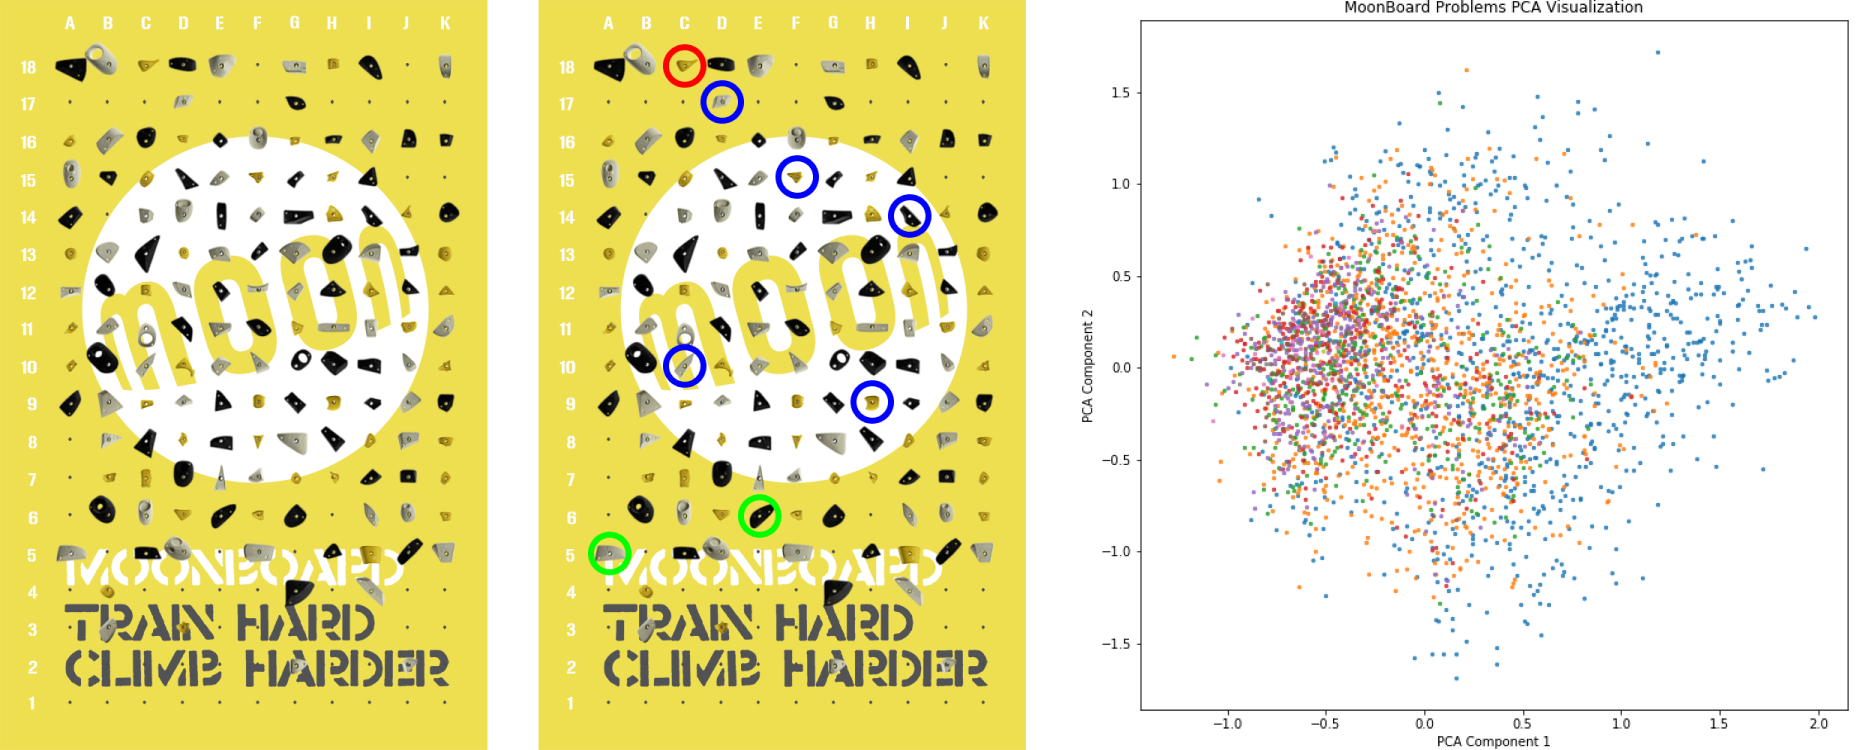
\includegraphics[width=.9\textwidth]{moondata}

\label{fig: MoonBoard data description}
\caption{(left) MoonBoard stock configuration (version 2016), (center) A specific MoonBoard route on the 2016 configuration, (right) Visualization of PCA decomposition of MoonBoard problems}
\end{figure}

% Methods Section
\section{Methods}
% GCN Subsection
\subsection{Graph Convolutional Network}
The Graph Convolutional Network as presented by \cite{kipf2016semisupervised} provides a framework by which node-level features can be combined with neighbors in a nonlinear transformation whose parameters are learned through backpropagation. Consider a graph $G = (V,E)$ where $V(\lvert V\rvert\ = n)$ and $E$ are the set of nodes and edges, respectively. Each node in $V$ is assumed to be connected to itself (self-adjacency) and is represented as a row in $X \in \mathbb{R}^{n \times m}$. Graph $G$ also has an adjacency matrix $A$ with a corresponding degree matrix $D$ where $D_{ii} = \sum_{j}A_{ij}$. A one-layer GCN featuring 1 convolution step is computed as
\begin{equation}
L^{(1)} = \rho(\widetilde{A}XW_{0})
\end{equation}
where $\widetilde{A} = D^{-\frac{1}{2}}AD^{-\frac{1}{2}}$ is the normalized symmetric adjacency matrix, $W_0 \in \mathbb{R}^{m \times k}$ is a weight matrix, and $\rho$ is an activation function. Note that $X$ can also be denoted as $L^{(0)}$. This one-step convolutional operation captures information about a node's immediate neighbors (Figure 2). By stacking multiple GCN layers, graph nodes can be embedded with features from neighbors successively further away,
\begin{equation}
L^{(j+1)} = \rho(\widetilde{A}L^{(j)}W_{j})
\end{equation}
where $j$ denotes the layer number.

\begin{figure}
\centering
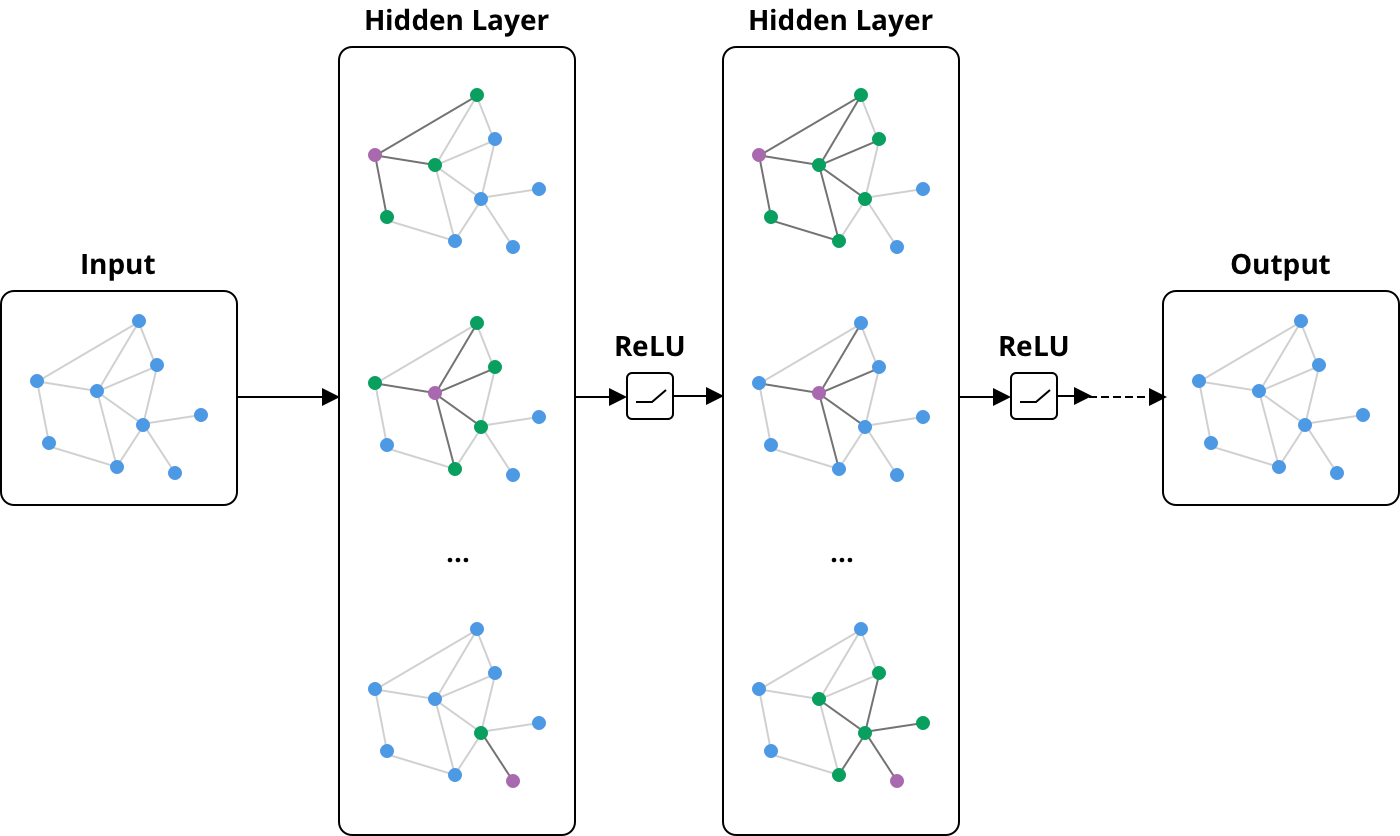
\includegraphics[width=.4\linewidth]{gcn_2steps}
\caption{At the first convolutional step, any node has access to its 1-hop neighbors. At the second convolution, nodes can "see" features from their 2-hop neighbors. Generally, $j$ convolution steps yields access to features from $j$-hop neighbors.}
\label{fig: Graph Convolutional Network}
\end{figure}

\begin{figure}
\centering
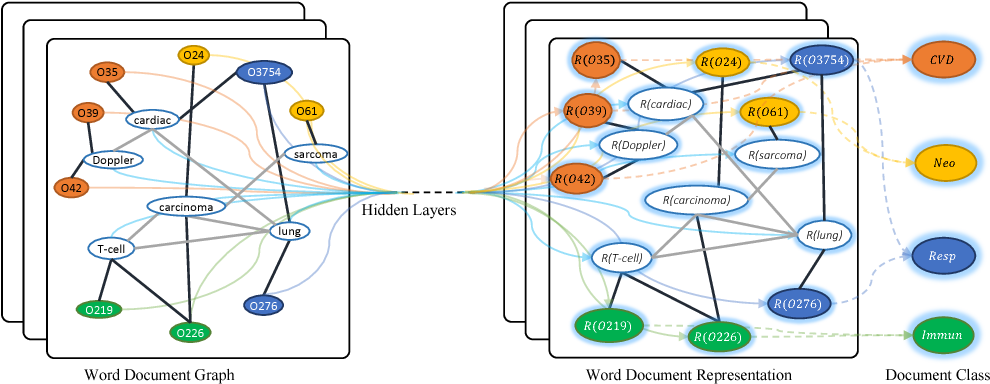
\includegraphics[width=.5\linewidth]{textGCN}
\caption{A heterogenous corpus graph for document classification using a Text GCN \cite{yao2018graph}. Nodes come in 2 types: document entities and word entities. The different colors correspond to different node categories (notice only document nodes are colored).}
\label{fig: Corpus graph for Text Graph Convolutional Network}
\end{figure}

% Text GCN Subsection
\subsection{Defining Adjacency and Text GCN}
Extending the vanilla GCN \cite{kipf2016semisupervised} to the Text GCN \cite{yao2018graph} involves framing graph $G$ as a heterogenous graph (Figure 3). In our MoonBoard application, an equivalence can be established between documents and problems --- words and holds. The adjacency matrix in such a graph is defined as
\begin{equation}
A_{ij}= 
\begin{cases}
    \text{PMI}(i, j), & \text{if } i, j \text{ holds} \\
    \text{IDF}(j), & \text{if } i \text{ problem } j \text{ hold} \\
    1, & \text{if } i=j \\
    0, & \text{otherwise}
\end{cases}
\end{equation}
where PMI of a hold pair $i, j$ is computed as
\begin{equation}
\text{PMI}(i, j) = \log\frac{p(i, j)}{p(i)p(j)}  \quad  p(i, j) = \frac{\#W(i, j)}{\#W}  \quad  p(i) = \frac{\#W(i)}{\#W}
\end{equation}
In Equation 4, $\#W(i)$ is the number of sliding windows over the problem corpus that contains the hold $i$, $\#W(i, j)$ is the number of sliding windows that contain both $i$ and $j$, and $\#W$ is the number of sliding windows total. For experimental purposes, we took two approaches in defining sliding windows: (1) over the scope of an entire problem (coined \texttt{PMI}) and (2) using a $5 \times 5$ filter (approximately half-armspan of an average climber) that slides over the canvas of a MoonBoard wall (Figure 1). Approach (2) was inspired by convolutional filters in CNNs and is coined \texttt{Win-PMI} for "Windowed" PMI.

Adapting Equation 2 to Text GCN for two steps of convolution on a multi-class classification task with ReLU activation, we get
\begin{equation}
Z = \text{softmax}(\widetilde{A}\,\text{ReLU}(\widetilde{A}XW_{0})W_{1})
\end{equation}
with an adapted cross-entropy loss function
\begin{equation}
\mathcal{L} = -\,\sum_{d\in\mathcal{Y}_P} \sum_{f=1}^{F} Y_{pf}\log Z_{pf}
\end{equation}
where $\mathcal{Y}_P$ is the set of MoonBoard problem indices that have labels and $F$ is the number of difficulty classes (11 in our case). This loss function only considers a subset of $V$ that are (1) problems and (2) have labels. Referencing Equation 5, two steps of convolution in a heterogenous problem-hold graph encodes an intuition of bridging problems to neighboring problems via shared holds. We expect these problem-hold-problem connections to significantly help in discriminating difficult routes from easy ones. 

% Discussion section
\section{Experiments, Results, and Discussions}
We ran a total of 17 experiments (see Table 1) that can be categorized into three broad categories: Baselines, Dense, and GCN. The Baselines category features a battery of classic statistical learning models. The Dense experiment category refers to a PyTorch implementation of fully-connected feed-forward networks and has two variations: Shallow and Deep, referencing the number of hidden layers in each network. The GCN family of experiments features several varieties and are prefixed by \texttt{GCN} under Table 1. Each successive tag describes (1) \texttt{(S)/(L)} the capacity of hidden layers as small or large, (2) \texttt{2S/4S} the number of convolution steps, (3) \texttt{OH/MH} one-hot or multi-hot features, and (4) \texttt{PMI/Binary/Self-Binary/Self-PMI/Win-PMI} adjacency tags. Tag \texttt{PMI} refers to Equation 3 (Approach 1), \texttt{Binary} refers to a version of Equation 3 where all non-zero values are set to 1, the \texttt{Self-} prefix denotes a version of adjacency where the diagonals of $A$ are re-set to identity after normalization to $\widetilde{A}$, and the prefix \texttt{Win-} identifies Equation 3 (Approach 2). 

% Table of results
\begin{table}[h!]
\centering
\caption{Summary of experiment results with per-class F1 scores and averaged accuracy, F1, and AUC scores}
\label{tab:my-table}
\begin{tabular}{@{}lccclccccc@{}}
\toprule
                            & \multicolumn{7}{c}{\textbf{Per-Class F1 Scores}} & \multicolumn{2}{c}{\textbf{Avg.}} \\ \midrule
\textbf{Experiment} & \textbf{V4} & \textbf{V5} & \textbf{V6} & ... & \textbf{V12} & \textbf{V13} & \textbf{V14} & \textbf{F1} & \textbf{AUC} \\
Logistic Regression         & 0.52  & 0.35  & 0.25  & ... & 0.22 & 0.00 & 0.00 & 0.23            & 0.70            \\
SVM                         & 0.53  & 0.40  & 0.31  & ... & 0.34 & 0.33 & 0.00 & 0.29            & 0.66            \\
Random Forest               & 0.66  & 0.36  & 0.26  & ... & 0.24 & 0.00 & 0.44 & 0.28            & 0.67            \\
Gradient Boosting           & 0.59  & 0.35  & 0.28  & ... & 0.27 & 0.25 & 0.00 & 0.27            & 0.62            \\
MLP                         & 0.58  & 0.38  & 0.34  & ... & 0.00 & 0.00 & 0.00 & 0.22            & 0.66            \\
Dense Shallow, MH           & 0.61  & 0.38  & 0.32  & ... & 0.37 & 0.00 & 0.00 & 0.26            & 0.67            \\
Dense Deep, MH              & 0.48  & 0.40  & 0.23  & ... & 0.21 & 0.00 & 0.00 & 0.22            & 0.65            \\
GCN (S) 2S, OH, PMI         & 0.36  & 0.28  & 0.22  & ... & 0.48 & 0.24 & 0.10 & 0.24            & 0.63            \\
GCN (L) 2S, OH, PMI         & 0.33  & 0.27  & 0.23  & ... & 0.48 & 0.25 & 0.13 & 0.24            & 0.64            \\
GCN (S) 2S, MH, PMI         & 0.57  & 0.38  & 0.33  & ... & 0.49 & 0.00 & 0.00 & \textbf{0.29}            & \textbf{0.73}            \\
GCN (L) 2S, MH, PMI         & 0.58  & 0.38  & 0.33  & ... & 0.45 & 0.00 & 0.00 & \textbf{0.29}           & \textbf{0.72}            \\
GCN (S) 2S, MH, Binary      & 0.54  & 0.38  & 0.33  & ... & 0.46 & 0.00 & 0.00 & \textbf{0.28}            & \textbf{0.72}            \\
GCN (S) 2S, MH, Self-Binary & 0.58  & 0.41  & 0.30  & ... & 0.14 & 0.00 & 0.00 & 0.25            & 0.70            \\
GCN (S) 2S, MH, Self-PMI    & 0.59  & 0.38  & 0.29  & ... & 0.56 & 0.00 & 0.00 & 0.27            & 0.68            \\
GCN (L) 4S, MH, PMI         & 0.52  & 0.34  & 0.33  & ... & 0.50 & 0.00 & 0.37 & \textbf{0.31}            & \textbf{0.73}            \\
GCN (S) 2S, MH, Win-PMI     & 0.55  & 0.37  & 0.33  & ... & 0.48 & 0.00 & 0.00 & \textbf{0.28}            & \textbf{0.73}            \\
GCN (L) 2S, MH, Win-PMI     & 0.57  & 0.38  & 0.34  & ... & 0.47 & 0.00 & 0.00 & \textbf{0.29}            & \textbf{0.72}            \\ \bottomrule
\end{tabular}
\end{table}

Referencing Table 1, the first observation is that GCN models using multi-hot features outperform baseline models and PyTorch Dense implementations across the board on averaged AUC. This result lends credibility to the effectiveness of utilizing nearby neighbors' features in classification tasks. Interestingly, amongst the best-performing models, using either \texttt{PMI}, \texttt{Binary}, or \texttt{Win-PMI} all seem to yield approximately equivalent results. This suggests that the connections amongst nodes themselves are more important than the weights of these edges. 

Additionally, we observe that the only GCN model featuring four convolutional steps yielded the best averaged F1 and AUC scores --- a surprising finding since the authors of \cite{yao2018graph} reported negligible performance gains after two GCN layers. This result suggests that there are meaningful relationships not only between MoonBoard problems sharing the same holds (1 degree of separation), but also in relationships 1 degree further. Intuitively, this might be interpreted as, "if my neighbors are mostly V5 \textbf{and} my neighbor's neighbors are also V5, I am likely to be a V5 as well."

\begin{figure}[h]
\centering
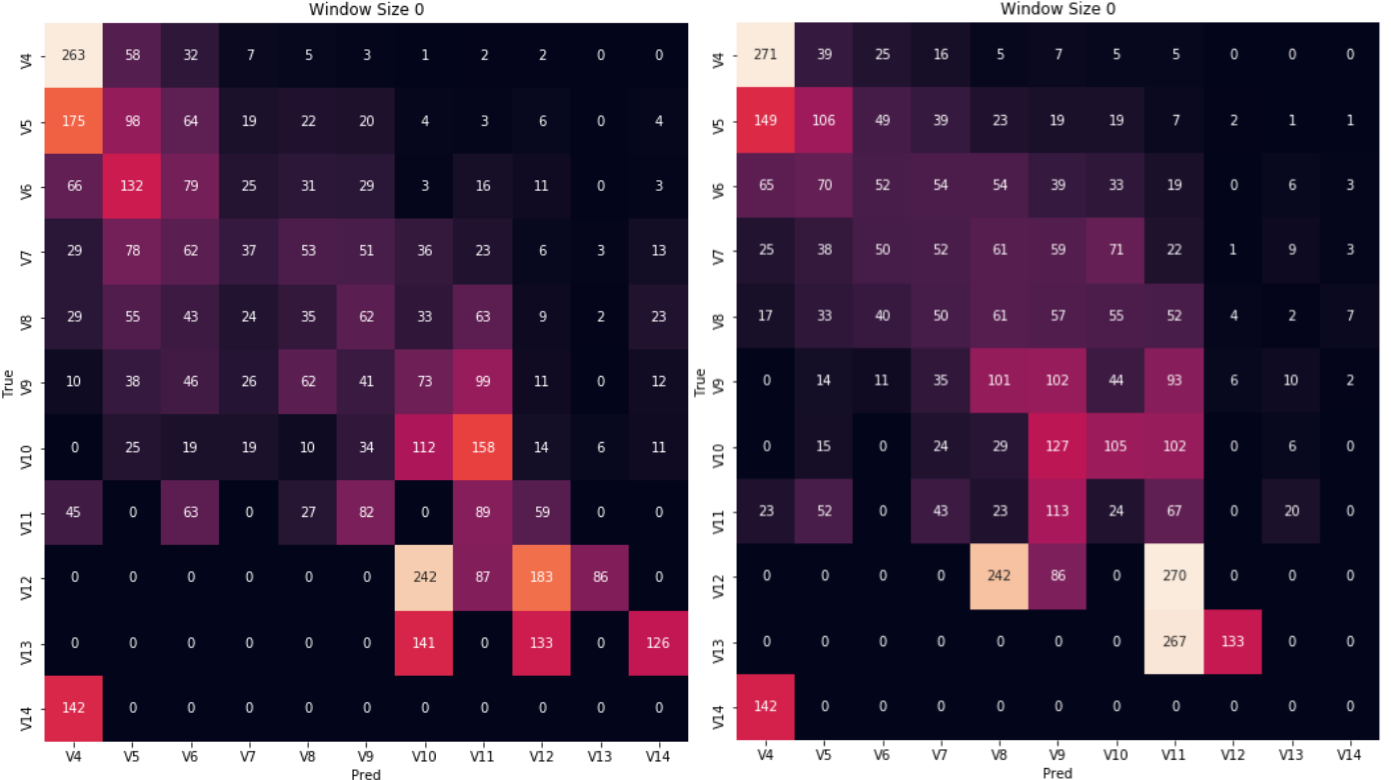
\includegraphics[width=.65\textwidth]{confusions}

\label{fig: Confusion matrices}
\caption{Confusion matrices on test data (left) GCN experiment multi-hot, 4 steps, regular PMI, (right) Logistic Regression. We can see that while logistic regression performs better near the lower-difficulty region, GCN is able to capture difficult problems more accurately.}
\end{figure}

Finally, referencing the two confusion matrices in Figure 4, we observe that it is really in the higher-difficulty classes where the 4-step GCN outperforms logistic regression. This behavior is well-aligned with our hypothesis that explicit graph connections better-enable label information to propagate to relevant neighbors even with a limited number of training samples. In this way, GCNs are far less susceptible to class imbalance than the classic machine learning algorithms or even fully-connected feed-forward networks.

% Conclusion Section
\section{Conclusions / Future Work}
In this work, we presented a novel application of graph convolutional networks to the rock climbing domain by adapting the Text GCN framework used in document classification. We found that GCNs, in conjunction with multi-hot feature embeddings, provide a signficicant improvement over classic statistical learning algorithms (i.e. logistic regression, random forest, etc...). Moreover, we also discovered that a 4-step graph convolutional operation yielded the best across-the-board results --- a finding that deviated from conclusions made by authors of TextGCN \cite{yao2018graph} and suggests that the optimal number of graph convolutions is highly domain-dependent. Finally, we validated that GCNs are indeed less susceptible to data imbalance, as compared with standard machine learning / deep learning algorithms. Given more time, we would've liked to explore a generative application \cite{mirza2014conditional} capable of producing a new Moonboard problem, given a user-specified difficulty.

% Contributions Section
\section{Contributions}
Cheng-Hao implemented the baseline statistical learning experiments, established evaluation metrics used to assess all models' performances, and maintained the project Github repository. Aaron assembled MoonBoard data, established an early GCN baseline, and created the balanced sampling protocol. Aaron and Cheng-Hao co-authored the PyTorch implementations of the Dense and GCN frameworks and co-planned the series of experiments to run. Aaron and Cheng-Hao both contributed to the drafting of this report. Rafael offered insights into alternative loss functions amenable to data imbalance on a graph network.

% References
\bibliographystyle{plain}
\bibliography{citations}

\end{document}